\documentclass[a4paper, 12pt]{paper}

\usepackage[portuges]{babel}
\usepackage[utf8]{inputenc}
\usepackage{amsmath}
\usepackage{indentfirst}
\usepackage{blindtext}
\usepackage{graphicx}
\usepackage[hidelinks]{hyperref}
\usepackage{gensymb}
\usepackage[top=2cm, bottom=2cm, left=3cm, right=2cm]{geometry}
\usepackage[table]{xcolor}
\usepackage{pbox}
\author{I. Messina, I. Abreu, P. Gil, R. Bellotti, T. Proux}

\title{Plano de Negócios - Minerva Atlética E-Sport}
\begin{document}
    \begin{titlepage}
    	\begin{minipage}[c][3cm][c]{3cm}
    		
\includegraphics[height=3cm]{img/ufrj_logo.png}
    	\end{minipage}
    	\begin{minipage}[c][3cm][c]{10cm}
    		Universidade Federal do Rio de Janeiro \\
    		Organização das Indústrias \\
    		Plano de Negócios
    	\end{minipage}
    	\begin{center}
    		\vspace{95pt}
    		
    		\huge{Plano de Negócios - Mineva Atlética E-Sport}
    		\vspace{260pt}
    	\end{center}
    	
    	\begin{center}
		    		  Ian Messina \\
			    	  Igor Abreu\\
			    	  Pedro Gil\\
			    	  Rafael Bellotti\\
			    	  Thasus Proux\\    			
    	\end{center}
    	
    	\begin{center}
    		\vspace{\fill}
    		Rio de Janeiro, 1 de Novembro de 2016
    	\end{center}
    \end{titlepage}
\newpage
\tableofcontents
\listoffigures
\newpage

\section{Plano de Gestão}
\subsection{Fatores Culturais}
Com os grandes avanços na área da tecnologia, os equipamentos eletrônicos estão cada vez mais presentes na nossa rotina e estão substituindo várias formas de interação entre as pessoas. As crianças estão entrando em contato com tablets e smartphones muito jovens e se interessando principalmente por jogos.\\
Por sua vez, a crescente capacidade dos computadores permite a criação de jogos com gráficos extremamente elaborados e a ascensão do mercado de jogos eletrônicos provoca jogos com enredos convidativos até mesmo a pessoas com idades mais elevadas.

\begin{figure}[!ht]
	\centering
	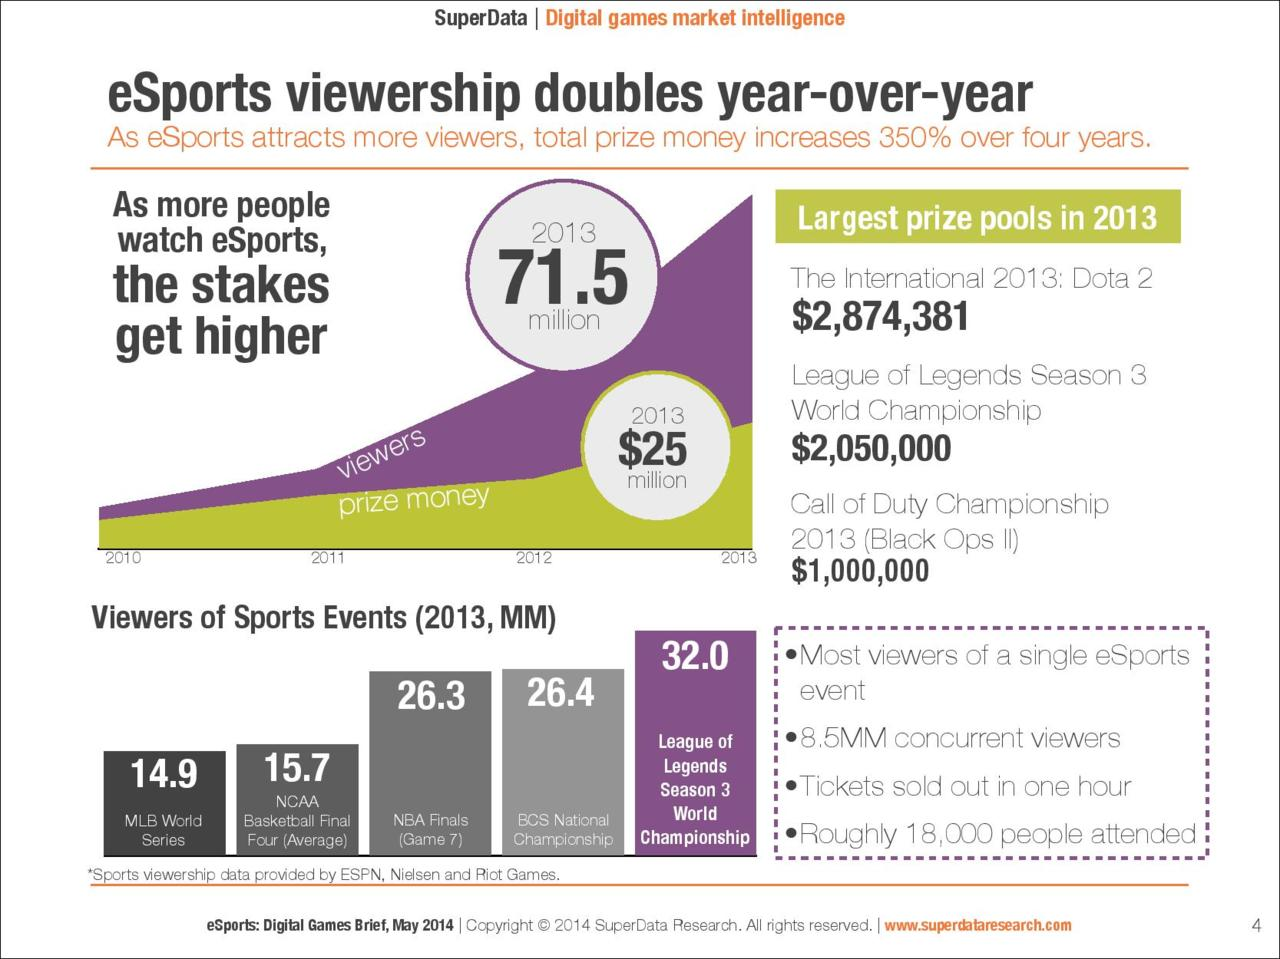
\includegraphics[scale=0.45]{img/img01.png}
	\caption{Crescimento do número de Telespectadores de eSport}	
\end{figure}
	
Com o crescimento de uma necessidade de novas formas de entretenimento, o acompanhamento de eventos de jogos eletrônicos se tornam uma opção alternativa de entretenimento para a população. O mercado de jogos eletrônicos está mundialmente em ascensão e deve gerar US\$ 99,6 bilhões até o final do ano. Este valor é 8.5\% maior que o do mesmo período no ano passado. A Newzoo, empresa que realizou a pesquisa, também prevê um crescimento positivo no Brasil: considerado o décimo primeiro país com maior mercado de jogos no mundo. Além disso, os dados da pesquisa apontam que dos 33,6 milhões de usuários brasileiros, 56\% investem dinheiro em jogos.\\
Essa vontade do brasileiro de estar mais imerso no mundo dos jogos, abre um espaço de demanda do mercado de trabalho. Onde a população deseja cada vez mais com o passar dos anos poder acompanhar melhor o cenário internacional e nacional de jogos eletrônicos competitivos. Considerando o cenário global, somente em 2013, havia 71.5 milhões de usuários assistindo jogos online.
\begin{figure}[!ht]
	\centering
	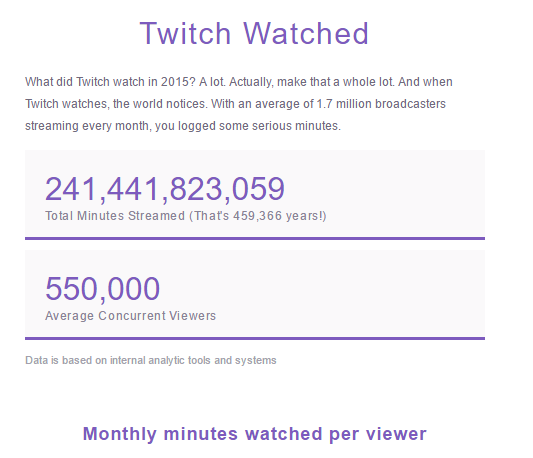
\includegraphics[scale=1]{img/img02.png}
	\caption{Dados sobre a plataforma de Streaming da Twitch}	
\end{figure}
Embora em crescimento, o cenário brasileiro necessita de mais eventos para atender a demanda desse mercado. Já que no cenário atual, os eventos são escassos, com uma necessidade de melhor organização em termos de qualidade e de relativamente pouco alcance.
\subsection{Fatores Ambientais}
Os eventos serão separados em etapas online e presenciais. As etapas online não apresentam diretamente nenhum impacto ambiental, pois seu conteúdo está atrelado ao meio virtual. Os eventos presenciais apresentam risco de poluição sonora, porém eles poderiam ser sediados em lugares de proteção acústica, podendo abaixar o risco até ser considerado nulo.
\subsection{Fatores Mercadológicos}
É considerado um consumidor em potencial todos que possuem um computador conectado à rede e que tenham interesse por jogos eletrônicos. A seguir será realizado uma análise dos principais agentes no mercado de jogos eletrônicos.
\subsubsection{Serviços de Streaming}
Serviços de streaming como Youtube e Twitch influenciam fortemente o mercado de jogos. Por se tratar das plataformas de acompanhamento de jogos em tempo real mais fortes no mercado, se torna indispensável considerar seus efeitos no mercado de jogos. \\
De acordo com a plataforma Twitch, a média de espectadores é de 550 mil e o número de minutos médios que cada espectador assiste usando a plataforma Twitch é de 421,6 por mês, já na plataforma Youtube foram 291 minutos por mês. O gráfico abaixo mostra o crescimento do número de espectadores e canais entre dia 20 de junho de 2012 e dia 29 de outubro de 2016 na plataforma Twitch.
\begin{figure}[!ht]
	\centering
	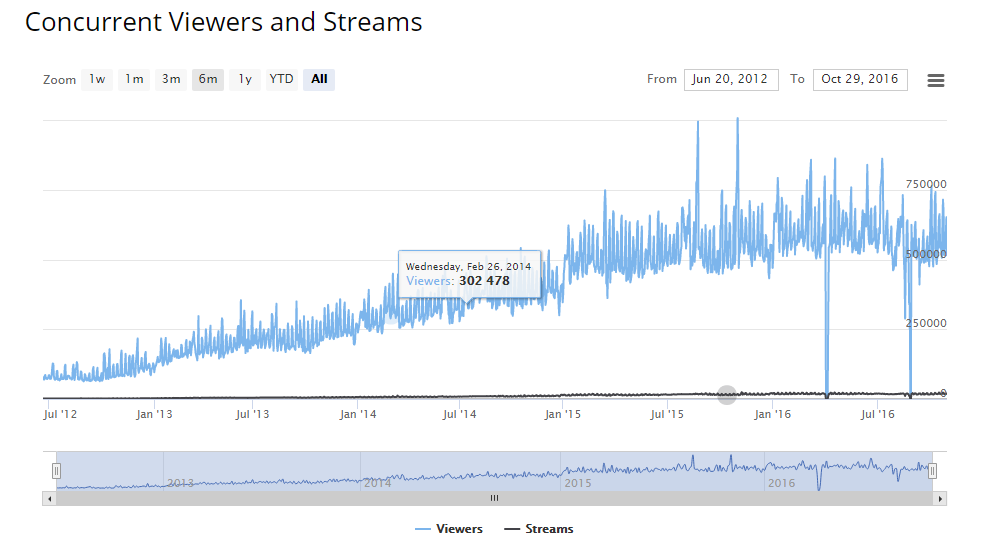
\includegraphics[scale=0.62]{img/img03.png}
	\caption{Aumento do número de telespectadores na plataforma de Streaming da Twitch}	
\end{figure}
\subsubsection{Eventos Presenciais}
Eventos presenciais reúnem espectadores e competidores em um espaço único, onde os espectadores podem assistir com seus próprios olhos os jogadores competindo no evento pelo primeiro lugar. Eventos são reconhecidos pelas empresas que criaram os jogos e geralmente ajudam na divulgação dos eventos em suas páginas e nas áreas de notícias dentro do portal do jogo. Eventos normalmente tem muito espectadores de esportes eletrônicos nos eventos, no caso do IEM Katowice foram mais de 104 mil espectadores somente no evento, ou seja, sem contar com os espectadores que assistiam por meio de televisão ou plataformas de streaming. Eventos como o DotA International 2016, que teve mais de 17 mil pessoas no evento, são eventos cujo valor da premiação vem de grande parte dos jogadores e espectadores. O valor da premiação para este evento chegou a 20.770.460 dólares americanos, o maior valor de premiação da história dos eSports, onde somente 1,6 milhões de dólares vieram da empresa Valve, criadora do jogo e responsável pela organização do evento.
\subsubsection{Televisão}
Embora ainda tenham pouco impacto no mundo da transmissão por televisão, os eSports estão crescendo nesse tipo de mídia. Atualmente, canais de grande nome como CNN estão cada vez mais investindo em jogos eletrônicos para atrair mais espectadores para seus canais de televisão. Além disso, a empresa ESL anunciou um canal de televisão dedicado a jogos eletrônicos chamado de esportsTV.
\subsection{Fatores Geográficos}
Os eventos puramente online não apresentam nenhuma barreira geográfica, porém pode gerar uma barreira para usuários de regiões com acesso à internet limitado. Por outro lado, os eventos presenciais requer que os espectadores estejam no evento fisicamente. Isto acaba gerando uma forte barreira geográfica, pois somente pessoas com condições financeiras favoráveis para bancar os custos de viagens, hospedagem e do evento em si, além de possuir tempo disponível poderão participar do evento.
\subsection{Fatores Políticos}
\subsection{Fatores Econômicos}
A economia do país está apresentando resultados surpreendentes com os poucos eventos que foram organizados. São Paulo sediou nos dias 26 a 30 de outubro de 2016 a quarta edição do torneio de CS:GO Pro League, premiando o primeiro colocado com US\$200 mil, sendo as premiações somadas igual a US\$750 mil.
\subsection{Fatores Sociais}
Uma grande parcela dos interessados nessas modalidades são jovens universitários ou mesmo adolescentes, sendo de vital importância não somente planejar eventos pensando nos calendários acadêmicos como também oferecer opções baratas de pacotes que cubram menos atividades durante o evento, mas que permitam jovens com recursos financeiros limitados de assistir aos jogos.
\subsection{Fatores Tecnológicos}
Todo o projeto é fortemente baseado em tecnologia, tanto eventos presenciais, como os não presenciais, desde a cobertura das partidas até a partida em si.
\subsection{Análise SWOT}
\subsection{Modelo de Negócio Canvas}
\subsection{Fatores Críticos de sucesso}
\newpage
\section{Plano de Marketing}
\subsection{Descrição dos Serviços}
\subsection{Forças do Marketing}
\subsubsection{Produto}
\subsubsection{Preço}
\subsubsection{Praça}
\subsubsection{Promoção}
\subsubsection{Pessoas}
\subsubsection{Processos}
\newpage
\section{Plano Operacional}
\subsection{Layout Operacional}
\subsection{Capacidade de Prestação}
\subsection{Processos Operacionais}
\subsection{Necessidade inicial de colaboradores}
\newpage
\section{Plano Financeiro}
\subsection{Investimentos Iniciais}
\subsection{Capital de Giro}
\subsection{Investimentos Pré-Operacionais}
\subsection{Investimento Total}
\subsection{Estimativa de faturamento}
\subsection{Estimativa do custo de comercialização}
\subsection{Estimativa do custo de cada produto vendido}
\subsection{Custos com Depreciação}
\subsection{Custos Operacionais}
\subsection{DRE}
\subsection{O Fluxo de Caixa}
\subsection{Indicadores de Viabilidade}
\subsection{Cenário Alternativo}
\newpage
\section{Estrutura da Empresa}
\subsection{Estrutura Organizacional}
\subsection{Estrutura jurídica}

\end{document}